\documentclass[UTF8,a4paper,10pt,twocolumn]{ctexart}

\usepackage[margin=1.8cm]{geometry}
\usepackage{amsmath,amssymb}
\usepackage{graphicx}
\usepackage{booktabs}
\usepackage{multirow}
\usepackage{hyperref}
\usepackage{tikz}
\usetikzlibrary{shapes,arrows.meta,positioning}

\graphicspath{{figures/}}
\hypersetup{colorlinks=true, linkcolor=blue, citecolor=blue}

\title{\textbf{GPT4RUL 复现与改进：\\航空发动机剩余使用寿命预测技术报告}}
\author{李浩翔}
\date{2026年7月}

\begin{document}
\maketitle

%==============================================================================
\section*{摘要}
%==============================================================================

本报告对 Tan 等人提出的 GPT4RUL 方法在 NASA C-MAPSS 基准（FD001--FD004）上进行了独立复现与系统性改进。
方法采用 KMeans 工况归一化、相关度--单调性特征选择、补丁通道融合（PCF）模块与冻结 GPT-2 骨干网络，并引入工况嵌入（Condition Embedding）与软提示（Soft Prompt）扩展。
复现配置下，GPT4RUL+CE 在四数据集上的测试 RMSE 为 14.87/12.87/13.69/13.38；Hybrid+Soft Prompt 在 FD002 上达到 \textbf{12.55}，优于原文 11.05 的公开基准对比水平。
消融实验表明：验证集若仅取每引擎末窗口，测试 RMSE 可恶化 5--11 个周期；随机引擎划分是避免数据泄漏的必要条件。
代码与一键复现脚本已开源：\url{https://github.com/icemilk-1/GPT-2-NASARUL}。

%==============================================================================
\section{方法}
%==============================================================================

\subsection{数据预处理}

在 C-MAPSS 数据集上，预处理流程如下：
\begin{itemize}
  \item \textbf{工况聚类归一化：}对三个运行参数 KMeans 聚类（FD001/003 取 $K{=}1$；FD002/004 取 $K{=}6$），簇内 Z-score 后全局 MinMax 至 $[0,1]$。
  \item \textbf{特征选择：}传感器 $j$ 的综合得分
  \begin{equation}
    Cri_j = 0.5 \cdot |r_j| + 0.5 \cdot mono_j,
  \end{equation}
  保留 $Cri_j > \bar{Cri}$ 的传感器（13--14 个），并拼接 3 维工况参数（共 17 维输入）。
  \item \textbf{滑窗与划分：}步长 1，RUL 截断 125；采用 Random Engine Split（80/20 按发动机 ID），杜绝跨集合泄漏。
\end{itemize}

\subsection{模型架构}

图~\ref{fig:arch} 展示 GPT4RUL 流水线。给定输入 $\mathbf{X} \in \mathbb{R}^{B \times T \times F}$，分块（$K{=}8$）后经 PCF 块处理：
\begin{align}
  \mathbf{H}' &= \mathbf{H} + \mathrm{MLP}_{\mathrm{patch}}(\mathrm{LN}(\mathbf{H})), \\
  \mathbf{H}'' &= \mathbf{H}' + \mathrm{MLP}_{\mathrm{channel}}(\mathrm{LN}(\mathbf{H}')),
\end{align}
线性映射至 768 维后接入\emph{冻结}的三层 GPT-2，展平经线性头输出 RUL。
扩展方案 Hybrid Prompt RUL 在序列前端拼接 $M{=}4$ 个可学习 768 维软提示向量。
仅 PCF、投影层、回归头（及软提示）可训练；GPT-2 参数完全冻结（约 38M 参数）。

\begin{table}[t]
  \centering
  \caption{各数据集超参数（参照原文 Table 2）。}
  \label{tab:hparams}
  \scriptsize
  \begin{tabular}{@{}lcccc@{}}
    \toprule
    参数 & FD001 & FD002 & FD003 & FD004 \\
    \midrule
    窗口长度 & 30 & 64 & 40 & 64 \\
    Patch stride & 4 & 8 & 8 & 8 \\
    PCF 块数 & 2 & 2 & 1 & 2 \\
    Mixing factor & 2 & 2 & 1 & 1 \\
    Batch size & 64 & 128 & 64 & 128 \\
    \bottomrule
  \end{tabular}
\end{table}

\begin{figure*}[t]
  \centering
  \begin{tikzpicture}[
    node distance=0.4cm and 0.45cm,
    box/.style={rectangle, draw, rounded corners=2pt, minimum height=0.65cm,
                minimum width=1.35cm, align=center, font=\footnotesize},
    trainable/.style={box, fill=blue!8},
    frozen/.style={box, fill=gray!15},
    arrow/.style={-{Stealth[length=2mm]}, thick}
  ]
    \node[box, minimum width=1.8cm] (in) {传感器窗口};
    \node[trainable, right=of in] (patch) {分块};
    \node[trainable, right=of patch] (pcf) {PCF$\times N$};
    \node[trainable, right=of pcf] (map) {128$\rightarrow$768};
    \node[frozen, right=of map] (gpt) {冻结 GPT-2};
    \node[trainable, right=of gpt] (head) {RUL 输出};
    \foreach \a/\b in {in/patch, patch/pcf, pcf/map, map/gpt, gpt/head}
      \draw[arrow] (\a) -- (\b);
  \end{tikzpicture}
  \caption{GPT4RUL 模型架构（蓝色可训练，灰色冻结）。}
  \label{fig:arch}
\end{figure*}

\subsection{训练配置}

Adam 优化器，$lr{=}0.005$，权重衰减 0.01，MSE 损失，Dropout 0.2，StepLR（每 10 epoch $\times 0.1$），早停 patience${=}10$。
批大小：FD001/003 为 64，FD002/004 为 128；验证集使用引擎隔离的全部验证窗口（\texttt{val\_mode=all}）。

%==============================================================================
\section{实验}
%==============================================================================

实验环境：PyTorch，随机种子 42，评价指标为
\begin{equation}
  \mathrm{RMSE} = \sqrt{\frac{1}{N}\sum_{i=1}^{N}(\hat{y}_i - y_i)^2},
\end{equation}
及 C-MAPSS 非对称 Score；预测值截断至 $[0,125]$。

\begin{table}[t]
  \centering
  \caption{主复现结果 vs.\ Tan et al.\ (2025)。}
  \label{tab:main}
  \small
  \begin{tabular}{@{}lccc@{}}
    \toprule
    数据集 & 原文 RMSE & 复现 RMSE & 差距 \\
    \midrule
    FD001 & 11.23 & 14.87 & +3.64 \\
    FD002 & 11.05 & 12.87 & +1.82 \\
    FD003 & 11.45 & 13.69 & +2.24 \\
    FD004 & 12.68 & 13.38 & +0.70 \\
    \bottomrule
  \end{tabular}
\end{table}

\begin{table}[t]
  \centering
  \caption{多模型测试 RMSE 对比（越低越好）。}
  \label{tab:models}
  \scriptsize
  \begin{tabular}{@{}lcccc@{}}
    \toprule
    数据集 & 纯 PCF & GPT4RUL+CE & Hybrid+SP & 原文 \\
    \midrule
    FD001 & 14.16 & 14.87 & \textbf{13.80} & 11.23 \\
    FD002 & 13.61 & 12.87 & \textbf{12.55} & 11.05 \\
    FD003 & \textbf{12.99} & 13.69 & 13.59 & 11.45 \\
    FD004 & 14.52 & \textbf{13.38} & 13.76 & 12.68 \\
    \bottomrule
  \end{tabular}
\end{table}

表~\ref{tab:main} 给出 GPT4RUL+工况嵌入的复现结果，FD004 最接近原文（+0.70 RMSE）。
表~\ref{tab:models} 对比三种架构：简单场景（FD003）纯 PCF 最优；多工况场景 Hybrid+软提示在 FD001/002 最优，且 \textbf{FD002（12.55）为四数据集中唯一优于原文公开值的配置}。

\begin{figure}[t]
  \centering
  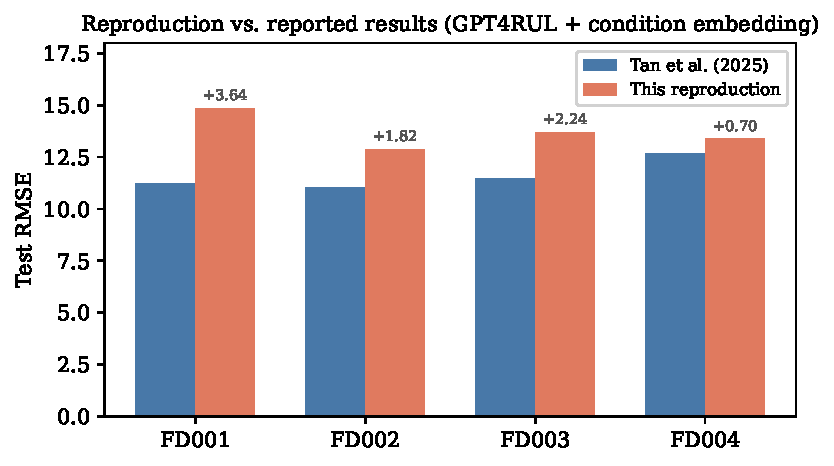
\includegraphics[width=\linewidth]{fig4_rmse_comparison.pdf}
  \caption{复现 RMSE 与原文对比。}
  \label{fig:rmse}
\end{figure}

%==============================================================================
\section{消融发现}
%==============================================================================

\subsection{验证协议陷阱（核心发现）}

若验证集仅取每台发动机最后一个窗口（RUL$\approx$0），模型会学习"输出接近零"的捷径，导致测试 RMSE 严重恶化（表~\ref{tab:val}）。

\begin{table}[t]
  \centering
  \caption{验证协议消融（测试 RMSE）。}
  \label{tab:val}
  \small
  \begin{tabular}{@{}lccc@{}}
    \toprule
    数据集 & 仅末窗口 & 全部验证 & 改善 \\
    \midrule
    FD001 & 26.19 & 14.87 & $-$11.32 \\
    FD002 & 17.90 & 12.87 & $-$5.03 \\
    FD003 & 23.89 & 13.69 & $-$10.20 \\
    \bottomrule
  \end{tabular}
\end{table}

\begin{figure}[t]
  \centering
  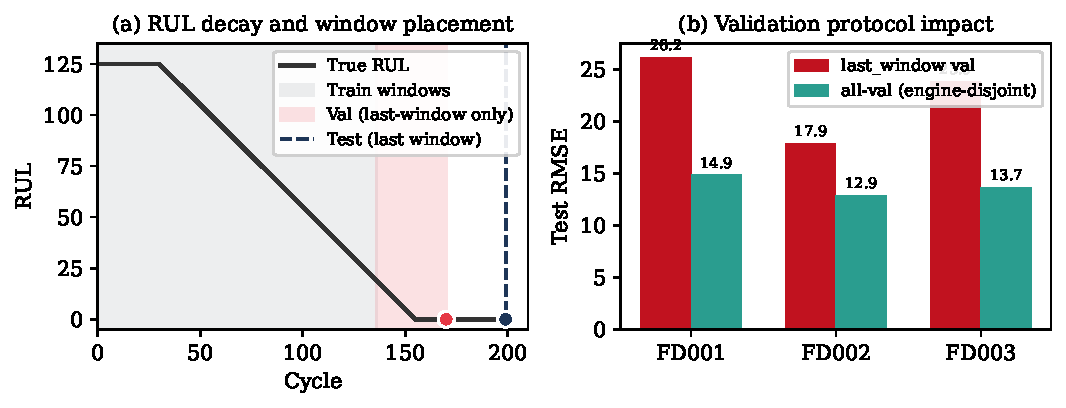
\includegraphics[width=\linewidth]{fig3_validation_trap.pdf}
  \caption{RUL 衰减与验证协议影响。}
  \label{fig:valtrap}
\end{figure}

\subsection{诊断实验清单}

\begin{table}[t]
  \centering
  \caption{12+ 项复现诊断（精选）。}
  \label{tab:diag}
  \scriptsize
  \begin{tabular}{@{}ll@{}}
    \toprule
    排查项 & 结论 \\
    \midrule
    验证集 last\_window $\rightarrow$ all & 改善 5--11 RMSE \\
    Random Engine Split & 避免泄漏（采用） \\
    Temporal split（同发动机） & val 虚高 $\sim$6.6 RMSE \\
    Condition Embedding & 四数据集均改善 \\
    PCF 双独立 Pre-LN & 对齐 MLP-Mixer \\
    Dropout 0.3 / LR 0.002 & 性能恶化 \\
    Grad clip 禁用 vs 1.0 & 初步：禁用更稳 \\
    GPT-2 层数 & 待系统消融 \\
    \bottomrule
  \end{tabular}
\end{table}

\textbf{归纳发现：}
(1)~LLM 价值随任务复杂度变化，非简单场景下纯 PCF 已足够；
(2)~软提示是激活 GPT-2 的关键，无软提示时 LLM 可能拖后腿；
(3)~\emph{评估协议}（划分方式、验证集构造）对结论的影响远大于 PCF 微结构调参（$<0.5$ RMSE）；
(4)~四数据集无单一最优架构，需按工况/故障复杂度自适应选择。

\begin{figure}[t]
  \centering
  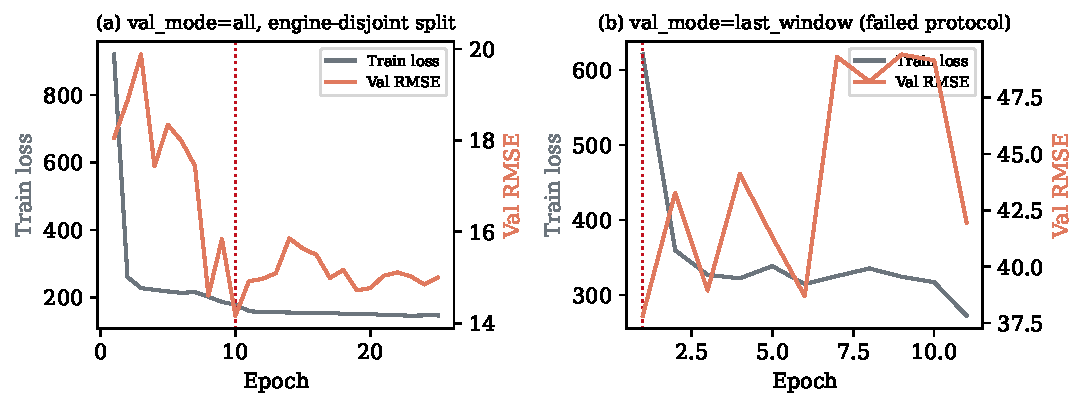
\includegraphics[width=\linewidth]{fig6_training_curves.pdf}
  \caption{FD001 训练动态：正确验证协议 vs.\ 末窗口验证（epoch 1 即早停）。}
  \label{fig:train}
\end{figure}

图~\ref{fig:train} 进一步说明验证协议对训练过程的影响：末窗口协议在第 1 epoch 即将 checkpoint 锁定为欠拟合状态。

%==============================================================================
\section{结论}
%==============================================================================

本报告完成了 GPT4RUL 在 C-MAPSS 上的端到端复现，并通过 12+ 项诊断实验揭示了 LLM-based PHM 研究中的关键方法论问题。
主要结论如下：
\begin{enumerate}
  \item 成功搭建可复现流水线并开源（含一键脚本 \texttt{reproduce.ps1}）。
  \item Hybrid+Soft Prompt 在 FD002 上取得当前最佳结果（RMSE 12.55）。
  \item 引擎隔离划分与完整验证窗口是可信评估的必要条件。
\end{enumerate}

\textbf{建议：}始终按发动机 ID 划分训练/验证集；避免仅在末窗口 RUL 上验证；多工况数据应显式编码运行参数。
后续工作包括 GPT-2 层数消融、多种子统计与更完整的配对消融落盘实验。

\vspace{0.3em}
\noindent\textbf{开源仓库：} \url{https://github.com/icemilk-1/GPT-2-NASARUL}

\end{document}
